\documentclass[useAMS,usenatbib]{mn2e}
\usepackage{amsmath,graphicx,bm,amsbsy,aas_macros,url,array,amssymb,breqn,aas_macros,todonotes,graphicx,comment}
\RequirePackage{fixltx2e}
\def\BCCP{$^2$}
\def\BCCPtxt{$^2$Berkeley Center for Cosmological Physics, University of California, Berkeley, Berkeley, California 94720, USA }

\def\ASU{$^7$}
\def\ASUtxt{$^7$Arizona State University, School of Earth and Space Exploration, Tempe, AZ 85287, USA}

\def\myemail{\altaffilmark{*}}
\def\myemailtxt{\altaffiltext{*}{aaronew@mit.edu}}

\def\UW{$^6$}
\def\UWtxt{$^6$University of Washington, Department of Physics, Seattle, WA 98195, USA}

\def\SKASA{$^8$}
\def\SKASAtxt{$^8$Square Kilometre Array South Africa (SKA SA), Park Road, Pinelands 7405, South Africa}

\def\RU{$^9$}
\def\RUtxt{$^9$Department of Physics and Electronics, Rhodes University, Grahamstown 6140, South Africa}

\def\CfA{$^3$}
\def\CfAtxt{$^3$Harvard-Smithsonian Center for Astrophysics, Cambridge, MA 02138, USA}

\def\ANU{$^{10}$}
\def\ANUtxt{$^{10}$Australian National University, Research School of Astronomy and Astrophysics, Canberra, ACT 2611, Australia}

\def\CAASTRO{$^{11}$}
\def\CAASTROtxt{$^{11}$ARC Centre of Excellence for All-sky Astrophysics (CAASTRO)}

\def\Haystack{$^{12}$}
\def\Haystacktxt{$^{12}$MIT Haystack Observatory, Westford, MA 01886, USA}

\def\MIT{$^1$}
\def\MITtxt{$^1$MIT Kavli Institute for Astrophysics and Space Research, Cambridge, MA 02139, USA}

\def\Curtin{$^{13}$}
\def\Curtintxt{$^{13}$International Centre for Radio Astronomy Research, Curtin University, Perth, WA 6845, Australia}

\def\Victoria{$^{16}$}
\def\Victoriatxt{$^{16}$Victoria University of Wellington, School of Chemical \& Physical Sciences, Wellington 6140, New Zealand}

\def\UWisc{$^{17}$}
\def\UWisctxt{$^{17}$University of Wisconsin--Milwaukee, Department of Physics, Milwaukee, WI 53201, USA}

\def\UMichigan{$^{18}$}
\def\UMichigantxt{$^{18}$University of Michigan, Department of Atmospheric, Oceanic and Space Sciences, Ann Arbor, MI 48109, USA}

\def\UMelbourne{$^{19}$}
\def\UMelbournetxt{$^{19}$The University of Melbourne, School of Physics, Parkville, VIC 3010, Australia}

\def\USydney{$^{14}$}
\def\USydneytxt{$^{14}$The University of Sydney, Sydney Institute for Astronomy, School of Physics, NSW 2006, Australia}

\def\CASS{$^{20}$}
\def\CASStxt{$^{20}$CSIRO Astronomy and Space Science (CASS), PO Box 76, Epping, NSW 1710, Australia}

\def\Tata{$^{21}$}
\def\Tatatxt{$^{21}$National Centre for Radio Astrophysics, Tata Institute for Fundamental Research, Pune 411007, India}

\def\RRI{$^{22}$}
\def\RRItxt{$^{22}$Raman Research Institute, Bangalore 560080, India}

\def\NRAO{$^{23}$}
\def\NRAOtxt{$^{23}$National Radio Astronomy Observatory, Charlottesville and Greenbank, USA}

\def\UWA{$^{24}$}
\def\UWAtxt{$^{24}$International Centre for Radio Astronomy Research, University of Western Australia, Crawley, WA 6009, Australia}

\def\ASTRON{$^5$}
\def\ASTRONtxt{$^5$Netherlands Institute for Radio Astronomy (ASTRON), PO Box 2, 7990 AA Dwingeloo, The Netherlands}

\def\Dunlap{$^{15}$}
\def\Dunlaptxt{$^{15}$Dunlap Institute for Astronomy and Astrophysics, University of Toronto, ON M5S 3H4, Canada}


\def\SNS{$^4$}
\def\SNStxt{$^4$Scuola Normale Superiore, Piazza dei Cavalieri 7, I-56126 Pisa, Italy}


\newcommand{\dtb}{T_b}
\newcommand{\Mpci}{\text{ Mpc}^{-1}}
\newcommand{\Mpc}{\text{ Mpc}}
\newcommand{\MHz}{\text{ MHz}}
\newcommand{\GHz}{\text{ GHz}}
\newcommand{\mJy}{\text{ mJy}}
\newcommand{\muJy}{ \text{ } \mu \text{Jy}}
\newcommand{\nJy}{\text{ nJy}}
\newcommand{\Msun}{ M_{\odot}}
\newcommand{\ssection}{$\S$}
\newcommand{\erg}{\text{ erg}}
\newcommand{\second}{\text{ sec}}
\newcommand{\yr}{\text{ yr}}
\newcommand{\degree}{^{\circ}}
\newcommand{\kperp}{k_\perp}
\newcommand{\kpara}{k_\parallel}
\newcommand{\mto}{$\to$}
\newcommand{\be}{\begin{equation}}
\newcommand{\ee}{\end{equation}}
\newcommand{\trans}{\mathsf{T}}
\newcommand{\mK}{\text{ mK}}
\newcommand{\K}{\text{ K}}
\newcommand{\meter}{\text{ m}}
\newcommand{\km}{\text{km}}
\newcommand{\hfine}{21\,cm}

\def\Let@{\def\\{\notag\math@cr}}


\bibliographystyle{mn2e}


\title{Simulations of the delay response of the HERA dish and implications for EoR power spectrum measurements.}
\author[A Ewall-Wice et al.]{A.~Ewall-Wice,\thanks{E-mail: aaronew@mit.edu}~
Jacqueline~N.~Hewitt,~
Richard~Bradley,~
Mariet~Venter,~
}


\begin{document}

\label{firstpage}
\pagerange{\pageref{firstpage}--\pageref{lastpage}}
\maketitle
\voffset=-.6in

\begin{abstract}
Numerical simulations of the spectral response of the PAPER feed+Dish+skirt antenna are performed. We find that the time-domain response of this arrangement misses the -60\,dB, 60\,ns spec by $\approx 25$\,dB. Simple calculations of foreground residual leakage into the EoR window are also carried out. After subtracting a perfect foreground model that does not include the antenna response, we find that the spectral structure extrapolated from the simulation causes foreground residuals to exceed the level of the cosmological signal $\sim 0.25h$Mpc$^{-1}$ beyond the wedge. Residuals for an antenna that meets the spec exactly are limited to $\sim 0.1h$Mpc$^{-1}$ beyond the wedge. While definitive conclusions about the overall contamination of the power spectrum should not be drawn from this analysis, we hope that it will motivate firmly established measurements of the HERA dish's performance and more thorough studies of the actual impact on foreground contamination in a full power spectrum pipeline analysis.
\end{abstract}


\section{CST time domain simulations.}
In this note, we simulate the effect of the time response function of the HERA dish power spectrum measurements. We run a 500\,ns CST simulation of the voltage response of the reciever to a 150\,MHz plane wave with a finite pulse envelope, incoming from zenith (${\bf v}_{in}$) and record the time domain voltage response at the receiver output (${\bf v}_{out}$). 



\begin{figure*}
\includegraphics[width=\textwidth]{figures/voltage.pdf}
\caption{The power in the voltage output as a function of time (green line normalized to 1 at $t=0$) in response to the power of our input plane wave (blue line) from our simulation. At 60\,ns, the power has only reached -35dB, significantly above the HERA spec.}
\label{fig:voltageResponse}
\end{figure*}


In Figure~\ref{fig:voltageResponse} we show the power (normalized to $t=0$) in the input wave and the voltage response. By 60\,ns, the power level has only fallen by $\approx -35$ dB. Since the input wave packet falls very steeply after $\sim 10$\,ns, we do not think that it is from the instantaneous reaction of the system to the falling plane wave. We can, of course, obtain the response function directly from the simulation by deconvolving the plane wave out of the total voltage output in a calculation that we now describe. 

\section{Deconvolving the response function}
The voltage a the receiver output terminals, $v_{out}$, may be expressed as the convolution of the antenna response function, $R(\tau)$ with the intput signal, $v_{in}$. 

\begin{equation}
v_{out}(t) = \int d \tau R(\tau) v_{in}(t - \tau) .
\end{equation}

Using the Fourier convolution theorem, we may undue this convolution by Fourier transforming, dividing the output by the plane wave, and fourier transforming back. Our estimate of the response, $\widehat{R}(t)$ may be expressed mathematically as 
\begin{equation}\label{eq:ftResponse}
\widehat{R}(t) = \boldsymbol{\mathcal{F}}^{-1}\left[ \frac{\boldsymbol{\mathcal{F}}{\bf v}_{out}}{\boldsymbol{\mathcal{F}}{\bf v}_{in}}\right]
\end{equation}
where
\begin{equation}
\boldsymbol{\mathcal{F}}_{kj} = e^{-2 \pi i kj /N}
\end{equation}
and
\begin{equation}
\frac{1}{N} \boldsymbol{\mathcal{F}}_{kj} = e^{2 \pi i kj /N}
\end{equation}




In Figure \ref{fig:tSim} we show the 500\,ns simulation of a plane wave incident on the HERA dish from zenith along with the voltage response. We also show the estimated response function out to $250$\,ns computed from equation \ref{eq:ftResponse}. Notable in the response function itself is very fine time scale structure that reaches positive and negative values but goes down very slowly as a function of delay. This noisy structure originates from the fact that our input plane wave is significantly smoother than time-resolution of the simulation and hence has compact support in the frequency domain. In Fig.~\ref{fig:freqDomain} we show the magnitude of the Fourier transform of the input plane wave (blue line) and see that it occupies a limited region of the frequency axis, centered at $150$\,MHz.  The voltage response (green line) is also primarily centered at the frequencies of the input wave (after all, it is effectively a multiplication of the input in the frequency domain) with significant numerical noise at frequencies away from the lobes and at the zero frequency region as well. The ratio of the unfiltered signals introduces significant high frequency noise power (red line). To eliminate the high frequeny noise, we multiply the frequency domain ratio of the voltage response and input wave by a $2$\,GHz FWHM Blackman-Harris window (cyan). After applying this first filter, the response function appears as the magenta line in the frequency domain. We show this noise filtered response function in Fig.~\ref{fig:tSimFiltered}. Even though significant modifications have been made in the frequency domain, the convolution of this response function with the input plane wave still well reproduces the voltage output. Another filter is ultimately applied to simulate the 100\,MHz instrumental bandpass and our final frequency-domain response is shown in Fig.~\ref{fig:finalFilter}.
%/Users/anguta/Documents/science/data/HERA_feed/reflectionGain.ipynb
\begin{figure*}
\includegraphics[width=\textwidth]{figures/deconvolution.pdf}
\caption{Simulated voltage levels from an input plane wave (blue line) as a function of time. The voltage response at the feed output (green line) is effectively the convolution of the input wave with the time-domain response function of the dish. We recover this response function by dividing the FFT of the voltage response with the FFT of the input plane wave and take the inverse transform to light red curve. We note that the measured response function only goes out to 250\,ns since an FFT deconvolution determines the response function between $-\tau/2$ and $\tau/2$ for a $\tau$ lenght simulation. In order to check our measured response function, we perform a direct convolution of the response with the input plane wave and recover the red points.}
\label{fig:tSim}
\end{figure*}



%/Users/anguta/Documents/science/data/HERA_feed/reflectionGainFix.ipynb
\begin{figure*}
\includegraphics[width=\textwidth]{figures/freq_domain.pdf}
\caption{The absolute value of the fourier transform of our input plane wave (blue line) and the voltage response (green line). The 150\,MHz plane wave, modulated by a gaussian only probes a finite region of frequency space while the voltage response outside of this region is dominated by numerical noise above $\sim 1$\,GHz. It is this numerical noise that leads to the fine time-scale structure in the unfiltered response function in Fig.~\ref{fig:tSim}. To remove this noise, we multiply the ratio of the voltage output to the plane wave intput (red line) by a Blackman-Harris window (cyan line) to obtain the filtered response function (black line).}
\label{fig:freqDomain}
\end{figure*}




\begin{figure}
\includegraphics[width=.48\textwidth]{figures/response_fft.pdf}
\caption{The absolute value of the Fourier transform of the response function convolved with a 100\,MHz Blackman-Harris window to simulate the actual HERA bandpass.}
\label{fig:finalFilter}
\end{figure}

\begin{figure*}
\includegraphics[width=\textwidth]{figures/deconvolution_filtered.pdf}
\caption{Same as Fig.~\ref{fig:tSim} except now the Fourier domain ratio between the voltage response and input plane wave is multiplied by a 2 GHz Blackman-Harris window. }
\label{fig:tSimFiltered}
\end{figure*}

\section{Considerations of filtering and sampling and the affect on the visibility.}
We have obtained an estimate of the response function from our simulations. However, the signal undergoes filtering and sampling, the effects of which we will consider here. 


Before being sampled, the signal is subjected to high and low-pass filtering to prevent aliasing. For HERA, the bandpass is centered at $\approx 150$\,MHz with a bandwidth of $\approx 100$\,MHz. The frequency response of the antenna after the analogue filtering step, $\widetilde{F}$ is 
\begin{equation}
\widetilde{v}_{out}(f) = \widetilde{R}(f) \widetilde{v}_{in}(f) \widetilde{F}(f)
\end{equation}
Sampling may be represented as multiplying the time-stream by a sampling function $s(t)$, 
\begin{equation}
s(t) = \sum_{m=-\infty}^{\infty} \delta_D(t-m \Delta t).
\end{equation}
Which corresponds to convolving with a Shah function in the Fourier domain. 
\begin{equation}
\widetilde{s}(f) =  \frac{1}{\Delta t} \sum_{m=-\infty}^{\infty} \delta_D \left(f - \frac{m}{\Delta t} \right)
\end{equation}
The F-step of the correlator takes place over a finite time interval which we will call $\tau$, leading to a convolution in the $f$ domain by a window function $\widetilde{W}_\tau(f)$. This window function is often quite narrow thanks to the employment of polyphase filtering. The output from the F-stage of the correlator, for the $i^{th}$ antenna, which we denote as $v_i$ is the input signal, multiplied by the antenna/analogue response function and the filter function and convolved with the sampling (shah) and the DFT window function. We assume in this note that all antenna have the same filter, sampling, and DFT window. 
\begin{equation}\label{eq:freqFull}
\widetilde{v}_i(f) = (( \widetilde{v}_{in}(f) \widetilde{R}(f) \widetilde{F}(f) ) \star \widetilde{s}(f) ) \star \widetilde{W}_\tau(f)
\end{equation}
For this analysis, we will assume that the analogue filter is sufficiently compact to prevent any aliasing and that the input spectrum $\widetilde{v}(f)$ along with the bandpass  is a constant over the width of $\widetilde{W}_\tau$. These two assumptions allow us to discard the convolutions in equation~\ref{eq:freqFull}
\begin{equation}
\widetilde{v}(f) \approx \widetilde{v}_{in}(f) \left[ \left( \widetilde{F} \widetilde{R} \right) \right](f) \equiv \widetilde{v}_{in}(f) \widetilde{g}
\end{equation}
Where $\widetilde{g}$ denotes the effective gain. If we assume that all antennas have the same response function, than the visibility formed from the product of two Fourier transformed voltage streams is
\begin{equation}\label{eq:vis}
v_{ij} = \widetilde{v}_i \widetilde{v}_j^* |\widetilde{F} \widetilde{R}|^2
\end{equation}
Strictly speaking, the delay response from the antenna element is a function of direction, and actually gives the frequency dependent beam in the direction of each source. 
\begin{equation}
v_{ij} = \int d \Omega I e^{2 \pi i {\bf b}_{ij} \cdot {\bf \hat{s}} } |\widetilde{F}|^2 A(f,{\bf \hat{s}})
\end{equation}
Where $|\widetilde{R}(f,{\bf \hat{s}})|^2$ is the beam of the antenna. In our analysis here, we are only considering the delay response to a plane-wave from zenith, so in predicting visibilities from this response, we are assuming that the antenna has the same frequency structure in all directions which is not in fact true. We are still in the process of simulating full beams and have run up against numerical precision issues.


For now, we assume $\widetilde{R}(f)$ is independent of direction and identical to the delay response function computed here. For $\widetilde{F}(f)$, we employ two Blackman-Harris windows with widths of $100$\,MHz centered at $150$\,MHz and $-150$\,MHz. This effectively eliminates any low frequency noise that may be present in our estimate of the response function as well. In Fig.~\ref{fig:dBresponse} we show the response function power level as a function of delay after applying this filter function. We see that it resembles a falling envelope multiplied by a $\sim$150\,MHz sinusoid. As we might expect from the voltage output in Fig.~\ref{fig:voltageResponse}, the power reaches $-35$\,dB at $\approx 60$\,ns. We also see that after $\approx 60$\,ns, the structure is dominated by lobed reflection structures that are spaced by $\approx 30$\,ns which corresponds to the round trip travel time between the feed and the bottom of the dish (which are separated by $\approx 5$\,m). 



\begin{figure*}
\includegraphics[width=\textwidth]{figures/responses_db.pdf}
\caption{The time-domain power response function of the PAPER feed with a 100 MHz blackman Harris window centered at 150 MHz applied. The response functions have been shifted $\approx 30$\,ns to the left to account for the initial propogation time for the input wave packet to arrive at the feed. We have drawn a dashed black line at 60\,ns to ephasize the HERA spec of -60dB at 60\,ns. We find ourselves at $\approx -35$\,dB at 60\,ns.}
\label{fig:dBresponse}
\end{figure*}



\section{Implications for Power Spectrum measurements}


Our analysis of CST simulations indicates that the HERA dish+PAPER dipole+skirt does not meet the -60dB at 60\,ns spec. In this section we try to address the implications on our ability to isolate foregrounds within the wedge and measure the 21\,cm power spectrum. To do this, we use a bandpass derived from the response function in our CST simulations and compute foreground visibilities with the reflections using equation \ref{eq:vis}. 

\subsection{Extrapolating the Response Function}

A critical limitation of our simulations is the limited extent of 250\,ns in the time domain. HERA is expected to have a frequency resolution of $\sim 100$\,kHz. To fully simulate the antenna gain to this resolution would require a simulation run on the order of $10^4$\,ns long, 40 times longer than its current length. As a result, we are forced to extrapolate the response function beyond $200$\,ns. While there is obviously enormous uncertainty in this extrapolation, the fact that the structure beyond $\approx 70$\,ns appears to be dominated by reflections provides us with a physically motivated framework for performing such an extrapolation; a wave having undergone $m$ reflections will decay in amplitude as $r^m$ where $r$ is the reflection coefficient. The number of reflections is proportional to delay, hence we  expect an exponential decay of the form
\begin{equation}\label{eq:pLaw}
R(\tau) \sim A r^\tau,
\end{equation}
for large $\tau$. We extrapolate the response function by tiling two reflection lobes from within the 250\,ns simulation span multiplied by a fit of equation \ref{eq:pLaw} to  the envelope for $t>70$\,ns. Interestingly enough, the best fit $r$ in our simulations for a 30\,ns reflection is quite large, $\approx 0.60$. In order to test the robustness of our extrapolation results, we also generate a response function with a time constant that is three times smaller than the fitted value, significantly accelerating the rate of reflection die off predicted by the simulaton. We also investigate whether the existing spec of -60\,dB at 60\,ns is sufficient in our simulations by scaling the simulated response function over 250\,ns by a power law that forces it to exactly exactly meet the spec and extrapolate as before. We show the extrapolated response functions for these three approaches in Fig.~\ref{fig:extrapolated}. We note that the extrapolated power law in the response function that meets the spec is less steep than the steep extrapolated power law. 



\begin{figure*}
\includegraphics[width=.33\textwidth]{figures/response_extrapolated.pdf}
\includegraphics[width=.33\textwidth]{figures/response_steep_extrapolated.pdf}
\includegraphics[width=.33\textwidth]{figures/response_spec_extrapolated.pdf}
\caption{Here we show the envelope of the magnitude of the response function convolved with a Blackman-Harris filter with FWHM $100$\,MHz centered at $150$\,MHz (blue points). We extend the simulation to arbitrary delays by copying the reflection structure from the simulation multiplied by an exponential (thick black line) to get the red line. We test the robustness of our predictions by decreasing the time constant by a factor of 3 (middle) and also scaling the simulated magnitudes by a power law so that they exactly meet the -60dB at 60\,ns spec (right).}
\label{fig:extrapolated}
\end{figure*}

\subsection{Simulations of Foreground Power Spectra}

From the extrapolated response function, we obtain an effective bandpass for the instrument by Fourier transforming into the frequency domain. We show the amplitude and phase of the effective bandpass in our fiducial extrapolation in \ref{fig:extBandpass}.


\begin{figure*}
\includegraphics[width=\textwidth]{figures/bandpass.pdf}
\caption{The bandpass between 100 and 200\,MHz calculated by taking the FFT of the 100\,MHz Blackman-Harris filtered response function extrapolated to $100\mu$s. }
\label{fig:extBandpass}
\end{figure*}


 We simulate visibilities with foregrounds in equation~\ref{eq:vis} by combining point sources from the MWACS catalogue \citep{HurleyWalker:2014} with the desourced Haslam map \citep{Remazeilles:2015} extrapolated to low frequency using a spectral index of $-0.5$. For the angular beam, we use an Airy function with a 14-m aperture. We generate visibilities for an E-W line 19 antennas phased to zenith with an LST of 4 hours and lat of -27 degrees, corresponding to the MWA EoR-01 field viewed from the MRO. We show our beam pattern and diffuse foregrounds in Fig.~\ref{fig:foregrounds}. 

\begin{figure*}
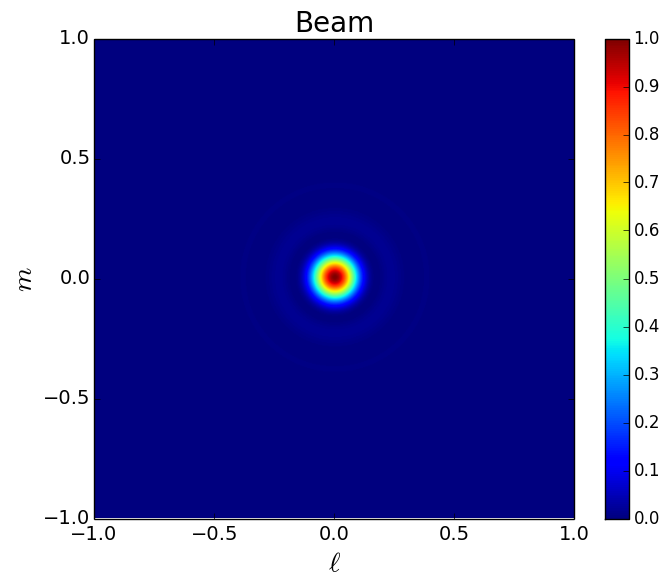
\includegraphics[width=.48\textwidth]{figures/beam.png}
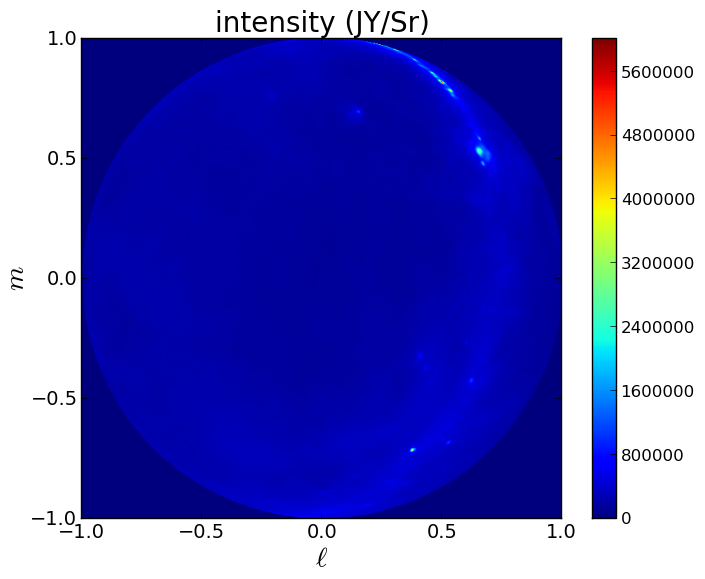
\includegraphics[width=.48\textwidth]{figures/diffuse.png}
\caption{The Airy primary beam used in these simulations (left) along with the diffuse foregrounds (right).}
\label{fig:foregrounds}
\end{figure*}


From these visibilities, we generate delay power spectra a-la \citep{Parsons:2014} using the formula
\begin{equation}
\widehat{P}(k) = \left( \frac{\lambda^2}{2 k_B} \right)^2 \frac{X^2 Y}{\Omega B} \left| \widetilde{V}(u,v,\tau) \right|^2,
\end{equation}
where $\lambda$ is the wavelength, $k_B$ is the Boltzmann constant, $\Omega$ is the effective beam solid angle given by $\Omega = \int A d\Omega$, $B$ is the bandwidth. $\widetilde{V}$ is the delay-transform of each visibility in frequency. 
\begin{equation}
\widetilde{V}(u,v,\eta) = \int d f V( {\bf b}f_0/c = {\bf u},f)e^{-2 \pi i f \tau}
\end{equation}
where $f_0$ is the center frequency of the band over which the delay transform is being taken. We perform the simulation over 16\,MHz centered at $150$\,MHz with a Blackman-Harris window applied to the DFT.  We show the foreground power spectra compared to 21cmFAST signal at $z=8$ In Fig.~\ref{fig:visPS} compared with the level of foregrounds for a flat bandpass smallest HERA baseline at $u_\lambda = 7.4$. To get a sense of how foreground subtraction without knowledge of the antenna spectral response might preform, we also form a power spectrum from the difference between visibilities with the spectral response of the antenna and a flat spectral response. We find that for the spectral response extrapolations that do not meet the HERA spec, the foreground residual is significantly above the level of the signal out to $k_\parallel \approx 0.2-0.25h$Mpc$^{-1}$. 


\begin{figure*}
\includegraphics[width=.33\textwidth]{figures/delay_response_compare.pdf}
\includegraphics[width=.33\textwidth]{figures/delay_response_compare_steep.pdf}
\includegraphics[width=.33\textwidth]{figures/delay_response_compare_spec.pdf}
\caption{The foreground power spectrum for the smallest HERA baseline with a flat bandpass (solid blue line) and the antenna response function (solid green line). The horizon + a 0.1 $h$Mpc$^{-1}$ buffer is denoted by the vertical black line. The residual visibility obtained from subtracting the foreground visibiliteis with a flat response function (as we might expect from model subraction) (red dashed line) is shown for our extrapolated response function (left), the steep response function (middle) and the response function forced to meet spec (right). For the response functions that do not meet the HERA spec, residuals after foreground subtraction remain above the signal level out to $k_\| \approx 0.2-0.25 h$Mpc$^{-1}$. In the response function that does meet the spec, residuals pass below the signal at $k_\| \approx 0.2 h$Mpc$^{-1}$.  }
\label{fig:visPS}
\end{figure*}

We next bin spherically to obtain 1d power spectra from our foreground subtracted visibilities, excluding the wedge plus a 0.07 $h$Mpc$^{-1}$ buffer. As we might expect from our smallest $u_\perp$ power spectrum, the spherical power spectra of foreground residuals with the response functions that do not meet the -60dB at 60\,ns spec exceed the signal at $k\gtrsim 0.2h$Mpc$^{-1}$ and only falling below $10\times$ the signal level at $0.25-0.30h$Mpc$^{-1}$ (Fig.~\ref{fig:ps1d}). 

\begin{figure*}
\includegraphics[width=.33\textwidth]{figures/hera_1dPower_EoR_feed.pdf}
\includegraphics[width=.33\textwidth]{figures/hera_1dPower_EoR_feed_steep.pdf}
\includegraphics[width=.33\textwidth]{figures/hera_1dPower_EoR_feed_spec.pdf}
\caption{Spherically binned power spectra excluding the wedge plus a 0.07 $h$Mpc$^{-1}$ buffer of the 21\,cm signal (black line) and the visibilities resulting from the subtraction of a foreground model without the delay response of the instrument (blue line). In the left panel, we show the residuals for the delay response extrapolated by an exponential, in the middle an exponential with a steep ($\times 3$ time constant, and the right, the response function scaled by a power law so that it meets the -60\,dB at 60\,ns spec.}
\label{fig:ps1d}
\end{figure*}


\section{The Efficacy of Delay Cleaning in the Presence of Reflections.}
In the previous sections, we considered the subtraction of a perfect foreground model with no knowledge of the Dish's spectral response. Since it is unlikely that a sub-percent accurate foreground model will exist in the near future, this assumption is highly unrealistic. We begin to replicate the expected foreground leakage in an actual analysis by simulating the foreground cleaning analysis employed bye PAPER. This work is ongoing and we describe some initial steps in this section. 

Foregrounds are simulated over a wide bandpass between 100 and 200\,MHz. Visibilities are Fourier transformed into delay space with a Blackman-Harris window function. The {\tt aipy.deconv.clean} method is used to clean with a delta function kernel within a clean box equal to the wedge plus a $0.1 h$\,Mpc$^{-1}$ buffer. The residuals are transformed back into frequency space and delay power spectra are formed from a 150-158\,MHz subband.

\begin{figure*}
\includegraphics[width=.48\textwidth]{figures/delay_response_compare_cleaned.pdf}
\includegraphics[width=.48\textwidth]{figures/delay_response_compare_cleaned_deep.pdf}
\caption{Left: The foregrounds power spectrum formed from a $150-158$\,MHz subband. Blue and Green lines denote the Foregrounds with and without the delay response of the dish respectively. The Dashed red line shows the power spectrum residual of the foregrounds while the cyan line shows the power spectrum residuals with the antenna response. Cleaning was performed with a tolerance of $10^{-3}$. We see that at $10^{-3}$ tolerance, the region of Fourier space that is foreground free is identical with and without the reflections but extends to $k \approx 0.3$\,$h$Mpc$^{-1}$. Right: The same as the left except cleaning is performed with a tolerance of $10^{-5}$. When cleaning much deeper, one is able to remove foregrounds to lower $k_\parallel$ however the reflections continue to contaminate out to $0.3$\,$h$Mpc$^{-1}$ regardless of the clean depth. }
\label{fig:PSCleaned}
\end{figure*}

 In Figure~\ref{fig:PSCleaned} we compare the residuals from cleaning with and without the delay response of the dish included. We find that the extent to wich the delay response matters depend heavily on the clean depth which will in turn depend on the level of integration performed before cleaning. If cleaning occurs with a tolerance of $10^{-3}$ then foregrounds, with or without the reflections, dominate the signal out to $k_\parallel \approx 0.3$\,$h$Mpc$^{-1}$. If cleaning with a tolerance of $10^{-5}$ occurs, than the foregrounds is performed, than without the reflection, the region of Fourier space down to $k_\parallel \approx 0.2$\,$h$Mpc$^{-1}$ opens up. We note that this requires the score difference between clean steps to be within an order of magnitude of the signal which is not expected to occur on a single baseline, even a redundant one. Integrating deeply enough on a single redundant baseline to perform such a clean may be a driver for expanding beyond HERA-331, even if the additional antennas do not directly add much sensitivity. 


\section{Conclusions and Caveats.}

Our numerical results show that the delay response of the HERA dish misses the -60\,dB at 60\,ns spec by a factor of $\sim 10^3$. While the choice of filtering function has a significant impact on our estimate of the response function, we have chosen a fairly conservative Blackman-Harris window and the actual voltage stream in response to the plane-wave input (Fig.~\ref{fig:voltageResponse}) agrees with our $-35$\,dB at 60\,ns estimate quite well. 

What is far more uncertain is the actual impact on the power spectrum. Our extrapolation framework is physically sensible and our predictions do not appear to change much with significant modifications to our extrapolation time constant, hence we consider our predictions robust against this degree of freedom. Our prediction of foreground contamination on the other hand, incorporates a very specific subtraction analysis that assumes perfect knowledge of the foregrounds and no knowledge of the frequency dependent gain; both incorrect assumptions for a real measurement. On the other hand, we have only considered the spectral response of the dish towards zenith and ignored the angular variation in the spectral structure of the beam which is likely to be more significant in the side-lobes (and closer to the edge of the wedge), leading us to believe that the projections here may actually be overly optimistic. 


\begin{comment}


We attempt to model the the full angular dependence of the frequency dependent gain in the next section, however the numerical resolution issues in CST's beam estimation lead us to be somewhat wary of these results. 

\section{CST simulations of the primary beam.}\label{sec:beamSim}

We investigate the full chromaticity of the PAPER feed+dish+skirt arrangement by computing the directivity of the X-polarized dipole arms in CST. The directivity is computed at spacings of 1 degree in polar coordinates $\theta$ and $\phi$ with 100\,kHz spectral resolution between 145 and 155\,MHz. Due to numerical precision issues, the frequency dependent gains computed in CST are found to have step-like structures on the order of several\,kHz wide. To circumvent this problem, we interpolate between beam slices that are 1\,MHz apart using both polynomial fitting (to 7th order) and cubic spline interpolation. Since the resolution issue can shift the beam values up to several hundred kHz, there may still be resolution-induced structure in the gains. In Fig.~\ref{fig:beamPlot} we illustrate the frequency structure of different lines of sight through the beam. After being fit to cubic-spline interpolated functions and 7th order polynomials, the delay transform of the frequency dependences does appear to exceed the level of a flat Blackman-Harris window by $\approx 20$\,dB at $k \approx 0.2$\,hMpc$^{-1}$, the region where we expect to obtain maximal EoR sensitivity. 


A significant problem with this calculation beyond the deficiency in frequency resolution and need for interpolation is the use of nearest neighbor interpolation of the primary beam in the angular direction. Since the delay transform mixes angular structure into frequency (which is a staircase in nearest neighbors), this could also cause nasty artifacts. 

\begin{figure*}
\includegraphics[width=\textwidth]{figures/beam_plot.pdf}
\caption{Left Column: line of sight cuts through simulations of the HERA XX-polarized primary beam derived using CST. The original simulations were run at 100\,kHz resolution, however the decimal point precision forces us to use interpolation between 1\,MHz slices. The dots show simulation points, solid lines indicate cubic spline interpolation and dashed lines denote 7th order polynomial fits which tend to have several \% residuals. In the middle column, we show the delay kernel of the LoS cuts. The thick black line indicates the enveloping Blackman-Harris window function. The polynomial and cubic-spline fits tend to produce excess power above 0.4 h/Mpc. In the right column we show the locations of our frequency cuts on the primary beam. }
\label{fig:beamPlot}
\end{figure*}




\begin{figure*}
\includegraphics[width=.48\textwidth]{figures/beam_poly_compare.pdf}
\includegraphics[width=.48\textwidth]{figures/beam_interp_compare.pdf}
\caption{(left): The power spectrum on the smallest HERA baseline for the polynomial interpolated beam (in frequency). (Right): The power spectrum on a single visibility with the cubic spline interpolated beam}
\label{fig:visBeam}
\end{figure*}
\end{comment}

\bibliography{ms}

\end{document}